\section{Description}
The exponential distribution is the probability distribution of the time between events in a Poisson point process, i.e., a process in which events occur continuously and independently at a constant average rate. It is a particular case of the gamma distribution. It is the continuous analogue of the geometric distribution, and it has the key property of being memoryless. In addition to being used for the analysis of Poisson point processes it is found in various other contexts.

% TODO
TODO: proof of memorylessness (see MIT notes)

\subsection{Probability mass function}
For $\alpha > 0$ and $p > 0$:
\[
	f(x) = \frac{\alpha^p}{\Gamma(p)} x^{p - 1} e^{-\alpha x}, \text{ for } x > 0
\]

Note that $f(x) > 0$ for $x > 0$ and:
\[
	\int_0^\infty f(x) \, dx = \frac{1}{\Gamma(p)} \int_0^\infty y^{p - 1} e^{-y} = 1
\]
because the definition of $\Gamma(p)$ is the valye of the last integral.

\begin{figure}[H]
	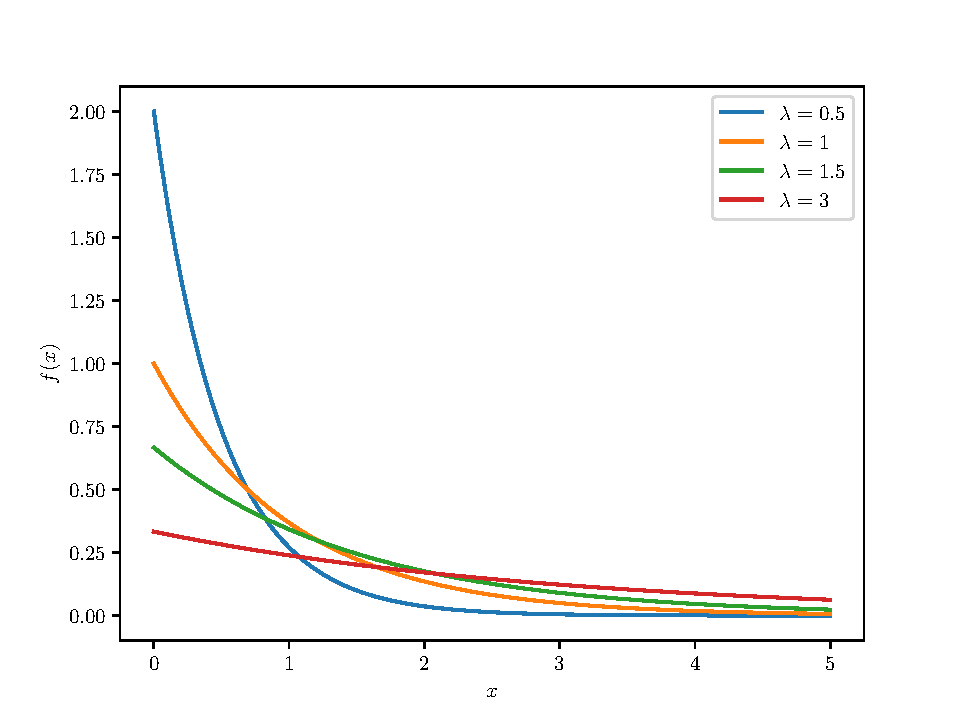
\includegraphics[width=\textwidth]{r/gamma/pdf.pdf}
	\caption{TODO: $f(x; \lambda) = \lambda e^{-\lambda x} \text{ if } x \geq 0$}
\end{figure}

\subsection{Cumulative distribution function}
For $\alpha > 0$ and $p > 0$:
\[
	F(x) = \int_0^x \frac{\alpha^p}{\Gamma(p)} t^{p - 1} e^{-\alpha t} \, dt \text{, for } x > 0
\]

\begin{figure}[H]
	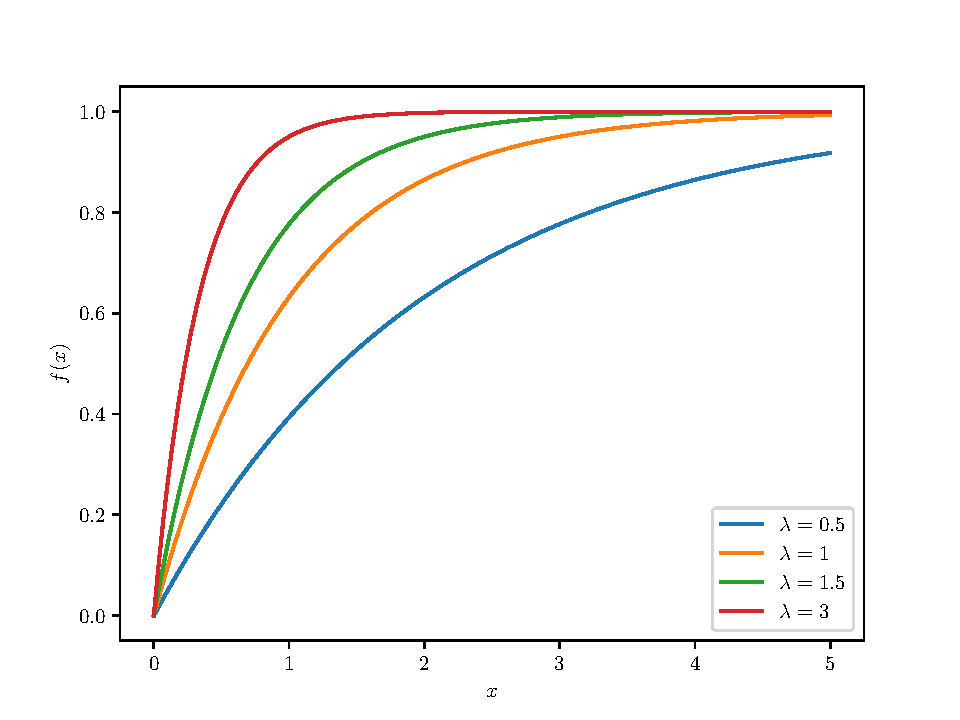
\includegraphics[width=\textwidth]{r/exponential/cdf.pdf}
	\caption{$F(x; \lambda) = 1 - e^{-\lambda x} \text{ if } x \geq 0$}
\end{figure}


\section{Moments}

\begin{tabularx}{\textwidth}{s X}
	\hline
	Mean & ?? \\\hline
	Variance & ?? \\\hline
\end{tabularx}


